%% 
%% Copyright 2019-2024 Elsevier Ltd
%% 
%% This file is part of the 'CAS Bundle'.
%% --------------------------------------
%% 
%% It may be distributed under the conditions of the LaTeX Project Public
%% License, either version 1.3c of this license or (at your option) any
%% later version.  The latest version of this license is in
%%    http://www.latex-project.org/lppl.txt
%% and version 1.3c or later is part of all distributions of LaTeX
%% version 1999/12/01 or later.
%% 
%% The list of all files belonging to the 'CAS Bundle' is
%% given in the file `manifest.txt'.
%% 
%% Template article for cas-dc documentclass for 
%% double column output.

\documentclass[a4paper,fleqn]{cas-sc}

\usepackage{subcaption}

\usepackage{multicol}

\usepackage[thinc]{esdiff} % for derivatives

% commands I use a lot
\usepackage{xspace}
\newcommand\thedata {$\{(t_i,h_{\text{obs}, i})\}_{i=1}^{N}$\xspace}
\newcommand\thedatanomath {\{(t_i,h_{\text{obs}, i})\}_{i=1}^{N}}
\newcommand\themodel {$h(t; h_0, \boldsymbol \alpha, \boldsymbol\theta)$\xspace}
\newcommand\themodelnomath {h(t; h_0, \boldsymbol \alpha, \boldsymbol\theta)}
\newcommand\thevars{h_0, \boldsymbol \alpha, \boldsymbol \theta, \sigma^2}

\usepackage{wrapfig}
% If the frontmatter runs over more than one page
% use the longmktitle option.

%\documentclass[a4paper,fleqn,longmktitle]{cas-dc}

%\usepackage[numbers]{natbib}
%\usepackage[authoryear]{natbib}
\usepackage[authoryear,longnamesfirst]{natbib}

%%%Author macros
\def\tsc#1{\csdef{#1}{\textsc{\lowercase{#1}}\xspace}}
\tsc{WGM}
\tsc{QE}
%%%

% Uncomment and use as if needed
%\newtheorem{theorem}{Theorem}
%\newtheorem{lemma}[theorem]{Lemma}
%\newdefinition{rmk}{Remark}
%\newproof{pf}{Proof}
%\newproof{pot}{Proof of Theorem \ref{thm}}


\begin{document}
\let\WriteBookmarks\relax
\def\floatpagepagefraction{1}
\def\textpagefraction{.001}

% Short title
\shorttitle{}    

% Short author
\shortauthors{}  

% Main title of the paper
\title [mode = title]{
Supporting Information: Scanning the cross-sectional area of a solid inside an opaque tank 
  via liquid level dynamics during draining
 }  

% Title footnote mark
% eg: \tnotemark[1]
\tnotemark[1] 

% Title footnote 1.
% eg: \tnotetext[1]{Title footnote text}
\tnotetext[1]{} 

% First author
%
% Options: Use if required
% eg: \author[1,3]{Author Name}[type=editor,
%       style=chinese,
%       auid=000,
%       bioid=1,
%       prefix=Sir,
%       orcid=0000-0000-0000-0000,
%       facebook=<facebook id>,
%       twitter=<twitter id>,
%       linkedin=<linkedin id>,
%       gplus=<gplus id>]

\author[1]{Gbenga Fabusola}%[<options>]

% Credit authorship
% eg: \credit{Conceptualization of this study, Methodology, Software}
\credit{}

% Address/affiliation
\affiliation[1]{organization={Oregon State University},
            % addressline={}, 
            city={Corvallis},
%          citysep={}, % Uncomment if no comma needed between city and postcode
            postcode={97331}, 
            state={Oregon},
            country={USA}}

\author[1]{Cory Simon}[orcid=0000-0002-8181-9178]

% Footnote of the second author
\cormark[1]

% Email id of the second author
\ead{Cory.Simon@oregonstate.edu}

% URL of the second author
\ead[url]{}

% Credit authorship
\credit{}


% Corresponding author text
\cortext[2]{Corresponding author}

% Footnote text
\fntext[1]{}


\renewcommand{\abstract}{} % Extremely risky!
\begin{abstract}
\end{abstract}
% For a title note without a number/mark
%\nonumnote{}
% Keywords
\maketitle



\section{Obtaining Torricelli's Law from Bernoulli's Equation}

\begin{wrapfigure}{r}{0.4\textwidth}
	\centering
	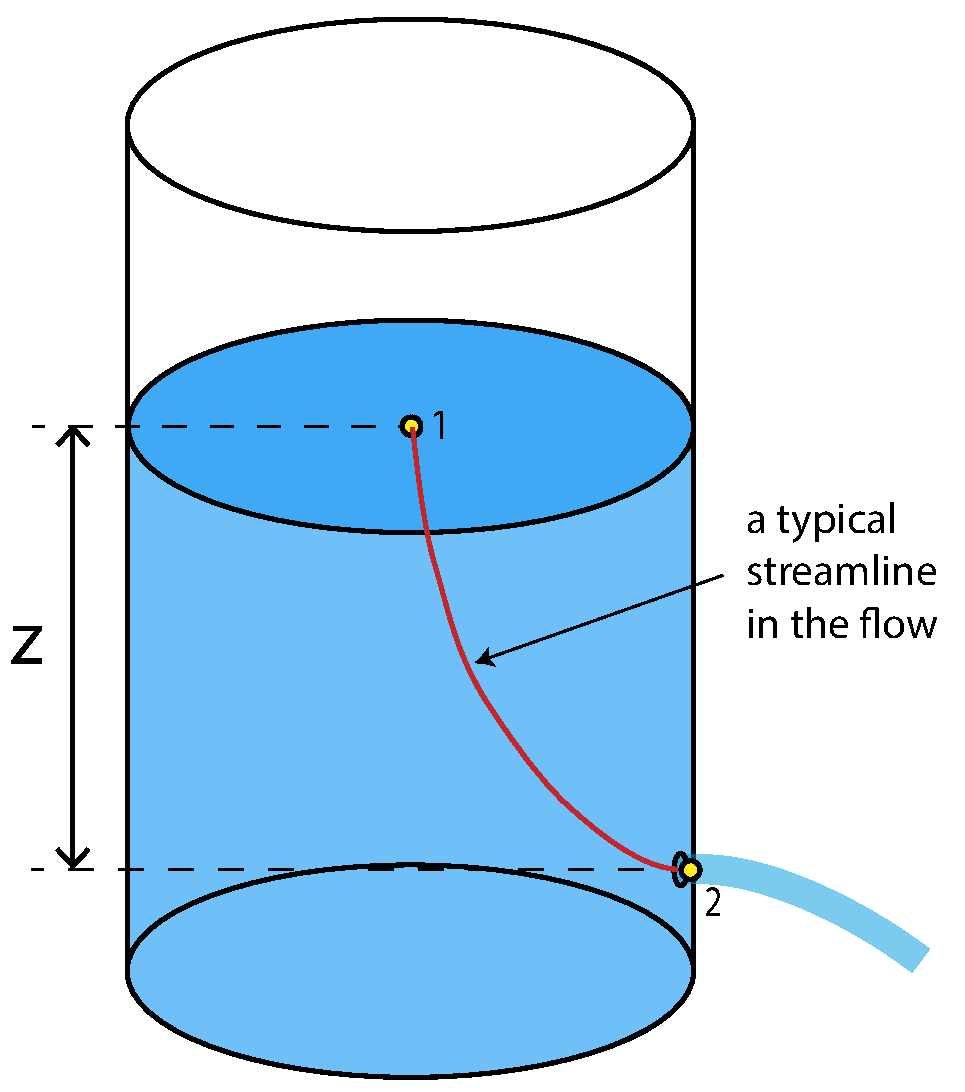
\includegraphics[width=0.4\textwidth]{../drawings_and_photo/torricelli_illustration.pdf}
\end{wrapfigure}

	Consider an open-top tank, nearly filled with liquid and with a small hole in its side that allows liquid to flow out of the tank to the atmosphere. 
	At some moment in time, we wish to find the velocity $v_2$ [m/s] at which the liquid ejects from the side of the tank, when the height of the liquid above the center of the hole is $z$ [m].
	
	To do so, we follow Bird, Stewart, and Lightfoot \cite{bsl_book} by applying Bernoulli's equation to two points in the liquid: 
	(1) a point just below the surface of the liquid at the top of the tank, near the center of the tank, and 
	(2) a point inside the outlet stream, just outside of the tank and near the center of the cross-section. 
	 Conceptually, we're considering a typical streamline of the flow extending from point (1) to point (2).
	We make three approximations: 
	(1) the flow along this streamline is at steady-state, which is a quasi-steady-state assumption that $z$ is approximately constant (despite dropping slowly),
	(2) the liquid is inviscid (neglecting frictional forces),
	and
	(3) the liquid is incompressible (constant density $\rho$ kg/m$^3$).
	(Also, the flow is isothermal.)
	
	A mechanical energy balance then implies Bernoulli's equation holds for the two points, which relates the velocity $v_i$ [m/s], pressure $P_i$ [N/m$^2$ $[=]$ kg$\cdot$ /(s$^2\cdot$m)], and elevation $y_i$ [m] of the liquid at the two points $i\in\{1,2\}$:
	\begin{equation}
	g y_1 + \frac{1}{2} v_1^2 + \frac{P_1}{\rho} = gy_2 + \frac{1}{2} v_2^2 + \frac{P_2}{\rho} 
	\end{equation}
	where $g$ [m/s$^2$] is the gravitational acceleration constant. 
	
	Now, since both points are at atmospheric pressure, $P_1=P_2$. And, we have $y_1-y_2=z$. Approximating $v_1\approx 0$ given the cross-sectional area of the liquid at the top of the tank is large relative to the size of the hole in the side of the tank, Bernoulli's equation reduces to:
	\begin{equation}
	g z  = \frac{1}{2} v_2^2,
	\end{equation}
	which states that the potential energy change of the liquid from point (1) to (2) matches the kinetic energy change. I.e., gravitational potential energy is converted to kinetic energy. Solving for $v_2$ gives Torricelli's law:
	\begin{equation}
	v_2 = \sqrt{2gz}.
	\end{equation}
% Biography
%\bio{}
% Here goes the biography details.
%\endbio

%\bio{pic1}
% Here goes the biography details.
%\endbio

\bibliographystyle{elsarticle-num}

% Loading bibliography database
\bibliography{refs}

\end{document}

